
\newif\iftwocol
\twocoltrue
%\twocolfalse

\iftwocol
	\documentclass[12pt,a4paper,twocolumn]{article}
	\newcommand{\imgscale}{0.26}
\else
	\documentclass[12pt,a4paper]{article}
	\newcommand{\imgscale}{0.52}
\fi	
	

\input{preamble}


\author{Mehmet Tekman}
\title{HaploHTML5: A Comprehensive Haplotype Resolution and Pedigree Creation Suite}


\begin{document}

\fontfamily{phv}
\fontsize{7pt}{9pt}
\selectfont\

\input{Abstract}

\section{INTRODUCTION}

Haplotype-phase inference is primarily set through Lander-Green derived linkage analysis programs that make use of a hidden Markov Model (HMM) approach (\citet{landergreen,kruglyak_parametric_1996}).

\begin{figure}[h]
\centering
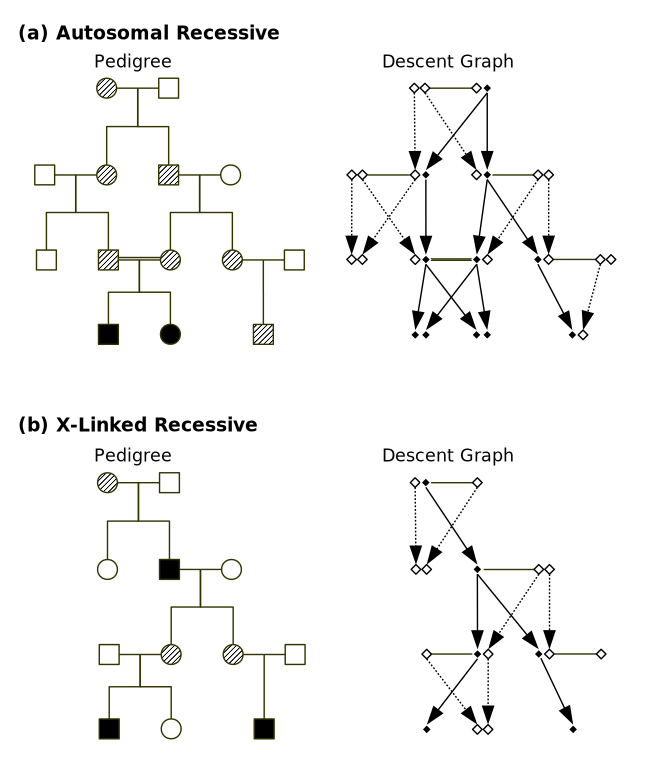
\includegraphics[scale=\imgscale]{descentgraph_both.png}
\caption{Descent graphs showing the path taken by disease vectors (bold arrows) and alleles (filled nodes). Carriers are shaded and Affecteds are filled, where both present the phenotype under dominant penetrance. [A2] Autosomal consanguineous pedigree; one of either parental alleles can be inherited. [B2] X-linked pedigree; Y-chromosomes (dotted nodes) restrict inheritance vectors.}
\end{figure}




programs are 

 - Genotyping chipsets (typically) unphased
 - Phase set through linkage
 - Linkage that operates using a Markov chain
 - Descent graphs

 - Previous haplotyping programs:
 	  - Pedigree/Draw (mamelka 1990)
 	  - CoPE (1999)
 	  - Pelican (Dudridge 2004)
 	  - HaploPainter (theile 2004)
 

\section{METHODS}
 - HaploPainter methodology
 - A* best-first
     - pseudocode
 - Javascript autoparallelization upon each chromosome due to independent appraisal (i.e. first pass creates dependencies, evaluation is chromosome non-dependent)




% Print biblio
% -- Must always have this otherwise document doesn't know where bib is.
\bibliography{bibs}
\end{document}